% !TEX root = mythesis.tex

%==============================================================================
\chapter{Hadron Spectroscopy on the Lattice}
\label{sec:spec}
%==============================================================================
% \newcommand{\todo}[1]{\textbf{\color{red}TODO: #1}}
\section{Background}
We first provide a brief overview of continuum QCD and how to extract low-energy observables using lattice QCD. In the following section we describe the nature of the so-called signal-to-noise problem which plagues calculations in LQCD, most notably the extraction of hadronic observables. As the Euclidean time between operators increases, the signal-to-noise ratio degrades exponentially. It is standard practice to use quark field smearing algorithms to circumvent this problem and ultimately extract ground-state energies with better statistics. Next, we introduce the mature method of distillation \cite{peardon_novel_2009} and the improvements to the signal of correlation functions in contrast to traditional smearing techniques. This will spell out the theoretical basis for the proceeding chapter on operator construction and the computational implementation of described methods to ultimately capture the mesonic and di-meson spectrum, setting the stage for exotic hadrons. 

\section{Continuum QCD}
QCD is the gauge theory of strong interactions with color $SU(3)$ as the underlying gauge group. The color degree of freedom was introduced into the quark model to satisfy the Pauli principle. The matter-fields in the theory are quarks (spin-$\frac{1}{2}$) fermions with six flavors and three possible colors (we don't detect these in experiment!). No quark has ever been observed as an asympotically-free state. During the 1970s, Gell-Mann\cite{Gell-Mann:1964ewy}and others \cite{PhysRevD.8.3633}\cite{PhysRevLett.31.494} tackled the question of exactly which symmetry of the quark model should be gauged. The ``hidden'' color degree of freedom possessed by quarks is plausible since we only observe color-singlets in nature. Thus, the strong forces between quarks with color need be colorless. Therefore, We can write down the QCD Lagrangian from the free-quark Lagrangian by applying the gauge principle with respect to the color gauge group $SU(3)$. The fundamental objects are the quark fields  $q_{\alpha,A}^{(f)}$ where $\alpha: 1,\dots,4$ are the Dirac-spinor indices, $f: 1,\dots,6$ denotes the flavor, and  $A: 1,2,3$ specifies the \text{color} index in the fundamental representation. 
The QCD Lagrangian is 
\begin{align}
    \mathcal{L}_{QCD} = \sum_{f=1}^{6} \sum_{a,b=1}^{3} \sum_{\alpha,\beta,\mu=0}^{3} \bar{q}_{\alpha a}^{(f)}(i(\gamma^\mu)_{\alpha \beta}(\mathcal{D}_{\mu;ab}) - m_f\delta_{\alpha \beta}\delta_{ab}) q_{\beta b}^{(f)} + \sum_{i=1}^{8}\sum_{\mu,\nu=0}^{3} -\frac{1}{4} G_{\mu\nu}^i G_i^{\mu\nu}
\end{align}
where $G_{\mu\nu} = \partial_\mu A_\nu - \partial_\nu A_\mu - ig[A_\mu,A_\nu]$ contains the gluons (gauge fields) $A_\mu = \sum_{a=1}^{8}A_\mu^a \lambda^a/2$ where $\lambda^a$ are the Gell-Mann matrices that index $1,\dots 8$ corresponding to the adjoint representation of $SU(3)$. The covariant derivative $\mathcal D_\mu$ acts on the quark fields like so $\mathcal D_\mu q_k = (\partial_\mu - igA_\mu)q_k$ 
$\mathcal{L}_{QCD}$ exhibits all the symmetries of the quark model and of course all discrete symmetries of the strong interaction, e.g. charge conjugation, parity, and strangeness(since the gluons are flavorless objects) \cite{Cheng1984GaugeTO}. These symmetries only become manifest via gauge invariance and renormalizability; In fact, $\mathcal{L}_{QCD}$ is derivable from the general form of the SU(3) Yang-Mills theory of quarks and gluons, see \cite{Cheng1984GaugeTO} for further details on this derivation. 

\subsection{Path integral formulation of QCD}
Wilson \cite{Wilson:1974sk} first introduced lattice gauge theory in 1974 where both space and time are discretized. The quantization of the gauge fields is done via a Wick rotation to Euclidean space $t\rightarrow i\tau$. We will arrive at this by starting with the real scalar free QFT in Euclidean space,
\begin{align}
    Z_{Eu.}[J] = \int D\phi \text{exp}{-\frac{1}{2} \int d^4x \phi^T(x)[\partial^2 +m^2] \phi(x) + \int d^4xJ^T(x)\phi(x)} 
\end{align}  
Now, when we discretize, $\phi(x)$ becomes a column vector 
$$\begin{bmatrix}
    \phi(x_1) \\
    \phi(x_2) \\
    \dots \\
    \phi(x_n)
\end{bmatrix} $$
which manifests as a massive dot product on a computer. 
$Z_{Eu.}[J]$ becomes $\text{exp}[\frac{1}{2}J^T D^{-1}J] Z[0]$ where
\begin{align}
    Z[0] = \tilde{\phi}(0) = \int d^4x e^{ipx} \phi(x)
\end{align}
In order to compute correlation functions, we need functional derivatives: 
\begin{align}
    \frac{\partial}{\partial J_y} \frac{\partial}{\partial J_x} Z[J] \rvert_{J=0} = D^{-1} 
    &= \braket{0|{\hat{\phi}(y)\hat{\phi}(x)}|0}
\end{align}
where the matrix element is again a time ordered product. In momentum space, the partition function is 
\begin{eqnarray}
    & Z_{Eu.}[J] = \int \underbrace{D\tilde{\phi}_p}_{\prod_{p_i} d\phi_{p_i}} \text{exp}[-\frac{1}{2} \int_x \int_p \int_{p'} \tilde{\phi}^T(p)[p^T +m^2] \tilde{\phi}(p) e^{i(p-p')x}] \\ 
    &= \int \prod_{p_i} d\phi_{p_i} \text{exp}[-\frac{1}{2}\tilde{\phi}^T(p_i)D_{p_i}\tilde{\phi}_{p_i}]
\end{eqnarray}
Using properties of Gaussian integrals, 
\begin{align}
    Z[0] = N \frac{1}{\sqrt{det(D)}}
\end{align}
with the Fermionic piece 
\begin{align}
    det(D) e^{J^TD^{-1}J}
\end{align}

Wilson's formulation of the Feynman path integral of QCD as a statistical mechanical sampling of the related Euclidean spacetime integral path 
\begin{align}
    Z_{QCD} = \int DA_\mu D\psi D\bar{\psi} \quad \text{exp}\left[-\int \bar{\psi}D[A_\mu]\psi - \frac{1}{4}\underbrace{G^2}_{\text{Gauge field Lagrangian}}\right]
\end{align}
We have to compute the Grassman numbers by hand 
\begin{align}
    Z_{QCD} = \int DA_\mu det D[A_\mu]e^{\underbrace{\frac{-1}{4}G^2}_{\text{Gauge action}}}
\end{align}
Which implies that for every configuration of ``Glue''(gauge fields), we have to know the value of the determinant. As we shall see, we don't actually evaluate this determinant, rather, we introduce ``pseudo-fermions'' into the QCD partition function 
\begin{equation}
    Z_{QCD} = \int DA_\mu D\phi^* D\phi e^{\left(\frac{-1}{4}G^2 - \phi^{*T}D_{A\mu}^{-1}\phi\right)}
\end{equation} where $D_{A\mu}^{-1}$ is a large sparse matrix with small eigenvalues. Now we have 
\begin{align}
    & \text{(Exactly solvable Gaussian)} \times \int d\phi d\phi^* e^{-\phi^*T D^{-1}\phi} \\ 
    &= \left(\frac{1}{det(D)}\right)^{-1} \\
    &= det(D)
\end{align}
which illuminates the large computational cost required of sparse matrix inversions, luckily, modern GPUs handle matrix multiplication well. Define an example Lattice universe of size $32^3 \times 96$ where $N_x=N_y=N_z = 32, \quad N_t=96$. Express 4D spacetime as a column vector: 
\begin{align}
   \underbrace{\psi(x)}_{field} = 32^3 \times 96 \times \underbrace{3}_{color} \times \underbrace{4}_{spin} = 12 \times 3145728 \quad \text{sites} 
\end{align}
The modus operandi is thus to manipulate matrices of this size with the computer. 
As a brief forary into the computational considerations, which will be further hashed out in the next chapter, consider the compute time of a matrix inversion: 
\begin{align}
    t_{cpu}\left(D^{-1} = \frac{\lambda_{max}}{\lambda_{min}}\right) \quad \text{(eigenvalues)} \\ 
    \lambda_{QCD}[D] \sim m_{u,d} \qquad ;\quad  m_{u,d} \ll \Lambda_{QCD} \ll \frac{1}{a} \\
    t_{cpu}[\text{volume}] \approx \left(\frac{L}{a}\right)^4 \frac{1}{am_q} \underbrace{\frac{1}{a}}_{\text{discretization penalty}} \sim \frac{1}{a^6}
\end{align}  
So we can deduce the scaling 
\begin{align}
    a \rightarrow \frac{1}{2}a \equiv 64 \times \text{orig}(t_{\text{cpu}})
\end{align} 
where the coarse graining of the lattice spacing $a$ is necessary in order to recover the continuum theory. With this formulation in hand, we can explicitly form the lattice gauge theory. 
Let 
\begin{align}
    S = \int d^4x \mathcal{L}(x) \\
    S_{LQCD} = \sum_{nm}^{} a^{n-4}\alpha_s^m S_{n,m} 
\end{align} where $n\geq4,m\geq0$. This is an expansion abotu the continuum limit, the first term in the expansion is exactly QCD. The remaining terms are the discretization effects resulting from the theory being transcribed in a finite box with boundary conditions. If we extrapolate to 0, we exactly recover the continuum theory of QCD. 
It needs to be emphasized that LQCD is \textbf{not} a model, rather, it is the only non-perturbative regularization scheme in the infrared regime that is systematically improvable, meaning one can dial the input parameters. This improvement manifests itself via the following properties of discretized spacetime, which are tightly coupled to high-performance computing architecture. The crucial feature of this discretized version of the continuum theory is gauge covariance, namely $m_{gluon} \rightarrow 0$, which is the only way the theory can remain renormalizable without adding new terms.  
\begin{itemize}
    \item Discretization scale ($a$) where there are no infinities at finite values of $a$
    \item Finite Volume 
    \item Unphysical quark mass, which allows us to extrapolate to the physical quark mass with effective field theory 
\end{itemize}


Discretization of a continuum theory naturally lends itself well to being transcribed onto a computer. In essence, we perform LQCD calculations on some HPC cluster, encode known properties of QCD into some EFT (e.g. Chiral perturbation theory, Baryon $\chi$PT, etc. which will not be discussed in this work) to make predictions about the standard model. The tunable parameters of LQCD simulations are the coupling constant $\alpha_s$ and the quark masses modulo the top quark.  Modern computing power allows us to perform these at the physical pion mass. 
\subsection{Discretization of the Fermion and Gauge Actions}
Wilson's goal was to quantize a gauge field theory on a discrete lattice in Euclidean space-time while preserving exact gauge invariance~\cite{Wilson:1974sk}. The expansion about the strong coupling constant requires summing over all possible quark paths and all surfaces that join these paths.  

Using results from general field theory, we can write down the following relation 
\begin{align}
    \braket{0|T{\hat{\phi}_N(x_N)\dots \hat{\phi}_1}(x_1)|0} \equiv\frac{1}{Z} \int D\phi\phi(x_N)\phi_1(x_1)e^{i\int d^4x\mathcal{L}(\phi,\partial\phi)}
\end{align}
We can write down the partition function $Z = \int D\phi e^{iS}$. 
The former is a time ordered-product of fields, which is hard to put on a computer but allows us to predict what we should see. The latter is composed of commuting numbers and an infinite dimensional integral over all gauge configurations, which we cannot naively calculate on a computer. However, we know that a computer, with suitable hardware architecture, can handle all IR non-pertrubative physics.   

We first need to discretize the hypercube into a grid with volume $N^4 = \text{number of sites}$ where $N$ is the spatial extent. Next, we perform a Wick rotation $t\rightarrow -i\tau$ to Euclidean spacetime so that the partition function becomes 
\begin{align}
    Z_{Eu.} = \int D\phi_{Eu.}\underbrace{e^{(-SE_u)}}_\text{Probability weight} 
\end{align} 
In order to find the most ``valuable'' configuration on our lattice, we must run a Monte Carlo simulation. This must satisfy the Ergodic hypothesis; The simulation must be able to run in both directions in Monte Carlo time. Now we can generate an ensemble of $\phi^i$'s 
\begin{equation}
    {\phi_{Eu.}^i: i-1,\dots N} 
\end{equation} that minimize the Euclidean action $S_{Eu.}$. Said another way, these are the trajectories that are as close to the classical action as possible; This is akin to how one can recover classical mechanics from quantum mechanics. 

% Integrating over Minkowski spacetime, we obtain the QCD action 
% \begin{align}
%     S_{QCD} = \int d^4x \{\underbrace{-\frac{1}{4} \sum_{a=1}^{8}F_{\mu\nu}^a F^{a\mu\nu}}_{S_G[A]}+ \underbrace{\sum_{f}\sum_{i,j=1}^{3}\sum_{\alpha,\beta=1}^{4}\bar{q}_{i,a}^f(x)[i(\gamma^\mu)_{\alpha\beta}(\mathcal{D}_\mu)_{ij} - m_f\delta_{ij}\delta_{\alpha\beta}]q_{j,\beta}^f(x)}_{S_f[A,\bar{q},q]}\}
% \end{align}
\section{Wilson's Lattice Quantization of Gauge Fields}
In this section we capture how Wilson defined the space-time integral of the QCD Lagrangian on a discrete lattice in Euclidean space-time. Put simply, the derivatives present in the continuum action are substituted with finite-differences and the integral over space-time is replaced with a sum over lattice sites. The action must be gauge invariant for any lattice spacing $a$. Fermion fields live at every lattice site $n$ $\phi(x) \rightarrow \phi_n$; We connect these fermions with oriented link variables (direction matters!) in order to retain gauge invariance. 
\begin{center}
    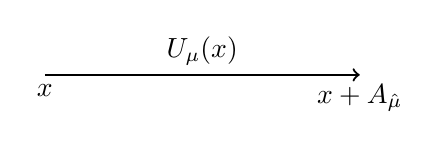
\begin{tikzpicture}
        \draw[->, thick] (0,0) -- (4,0);
        \node at (0,0) [below] {$x$};
        \node at (4,0) [below] {$x+A_{\hat{\mu}}$};
        \node at (2, 0.3) {$U_\mu(x)$};
    \end{tikzpicture}
    \end{center}

% Plaquette
\begin{center}
    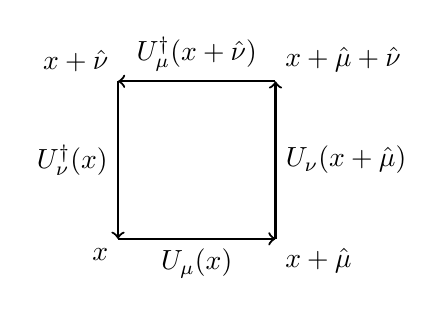
\begin{tikzpicture}
        \draw[->, thick] (0,0) -- (2,0) node[midway, below] {$U_\mu(x)$};
        \draw[->, thick] (2,0) -- (2,2) node[midway, right] {$U_\nu(x+\hat\mu)$};
        \draw[->, thick] (2,2) -- (0,2) node[midway, above] {$U_\mu^\dagger(x+\hat\nu)$};
        \draw[->, thick] (0,2) -- (0,0) node[midway, left] {$U_\nu^\dagger(x)$};
        
        \node at (0,0) [below left] {$x$};
        \node at (2,0) [below right] {$x + \hat\mu$};
        \node at (2,2) [above right] {$x + \hat\mu + \hat\nu$};
        \node at (0,2) [above left] {$x + \hat\nu$};
    \end{tikzpicture}
    \end{center}

    
The fundamental square of a hypercubic lattice is the plaquette, $U_{\mu\nu}(x)$ is an oriented square. The trace of  $U_{\mu\nu}(x)$ is a gauge-invariant object, thereby allowing the gauge-field piece of the action in lattice units  
\begin{equation}
    U_{\mu\nu}(x) = \text{Tr} \left[ U_\mu(x) U_\nu(x + \hat{\mu}) U_\mu^\dagger(x + \hat{\nu}) U_\nu^\dagger(x) \right]
\end{equation}
The wilson gauge action, simple and unimproved, is a sum over all plaquettes
\begin{align}
    S_G[U] = \frac{2}{g^2} \sum_{n\in\Lambda}^{}\sum_{\mu < \nu}^{} Re\left(Tr\left[\mathbb{I} - U_{\mu\nu}(x)\right]\right)
\end{align}
where the coefficient is the inverse gauge coupling. 
In Euclidean space, this becomes 
\begin{align}
    S_G[A] = \frac{1}{2g^2} \int d^4x Tr\left[F_{\mu\nu}(x) F_{\mu\nu}(x)\right]
\end{align}
We take the trace over color indices because the gluon fields are matrix valued, which keeps the action invariant under gauge transformation. To recapitulate, we have the following now at our disposal:
\begin{itemize}
    \item $U_\mu(x)$ is a link variable connecting sites $x, x+\mu$ 
    \item Gauge transformation $U_\mu(x) \to U'_\mu(x) = \Omega(x)U_\mu(x)\Omega(x+\hat{\mu})^\dagger$
\end{itemize}
Where the gauge fields $U_\mu(x)$ and $\Omega(x)$ are both elements of $SU(3)$ on each lattice site. 
We want to define a lattice gauge transporter with these attributes. In the continuum, a candidate that possess such properties would be a path-ordered exponential integral of the gauge field $A_\mu$ along some curve $C_{xy}$ that connects the points $x,y$ 
\begin{equation}
    G(x,y) = p\cdot \exp\left(ia\int_{C_{xy}}^{}A_\mu(x) \cdot ds\right)
\end{equation},
so we need a link variable $U_\mu(x) = G(x,y) + \sigma(a)$ where $\sigma(a)$ are the higher order corrections. Wilson's choice was 
\begin{equation}
    U_\mu(x) = \exp\left(iaA_\mu(x)\right)
\end{equation}
Therefore, by defining a link variable, we restore the gauge invariance. If we did not, then the gluon would be massive. Now we can write down what is called the \textit{Symanzik Expansion} 
\begin{equation}
    \lim\limits_{a \to 0} S_{LQCD} = S_{QCD} + \underbrace{aS_{LQCD}^5 + a^2 S^6_{LQCD}}_{\text{discretization corrections}}
\end{equation} where the lattice spacing $a = \frac{1}{\Lambda_{\mu\nu}}$. We can systematically control the above discretization errors by generating ensembles with various lattice spacings. 

This formulation begs the question; We have been working in Euclidean space, why can we not just use Minkowski space? The action in Minkowski is a wildly oscillating integral 
\begin{equation}
    Z_\mu = \int DA_\mu \det\left[D[A_\mu]\right] e^{i \sum_{x}^{}\frac{1}{4}G_{\mu\nu}G^{\mu\nu}}
\end{equation}
with no known algorithm to solve it. However, back in Euclidean space, we have 
\begin{equation}
    Z_{EU} = \int DA_\mu \det\left[D[A_\mu]\right] e^{- \sum_{x}^{}\frac{1}{4}G_{\mu\nu}^{EU}G_{\mu\nu}^{EU}}
\end{equation} where the term in exponentiated sum is $S_G$ or $S - \text{"glue"}$. $e^{-S_G} \in \mathbb{R}$ so we can use Monte Carlo probability sampling to determine which $G$'s are important, namely those which minimize the classical action. Moreover, we don't want to wick rotate back to Minkowski space $-i\tau \to t$, all physics can be extracted from Euclidean space. The hadron spectrum can be easily computed, but we cannot compute scattering processes directly in Euclidean space (this is where the L\"{u}scher Quantization condition enters). 

Finally, we take Wilson's choice $U_\mu(x) = \exp\left(iaA_\mu(x)\right)$ and insert it into the expression for the plaquette $U_{\mu\nu}(x)$ and apply the Baker-Campbell-Hausdorff theorem\cite{Hall2004LieGL} to obtain the expression for the plaquette 
\begin{equation}
    U_\mu\nu(x) = \exp\left(ia^2F_{\mu\nu}(x) + \mathcal{O}(a^3) \right)
\end{equation} where $F_{\mu\nu}(x) = -i\left[D_\mu(x),D_\nu(x)\right]$ is a commutator of covariant derivatives. 

The \textbf{Lattice version of the fermion action} is
\begin{equation}
    S_F^0 = a^4 \sum_{x\in\Lambda}^{} \bar{\psi}(x)\left(\sum_{\mu=1}^{4} \gamma_\mu \frac{\psi(x+\hat{\mu}) -\psi(x-\hat{\mu}) }{2a} + m\psi(x)\right)
\end{equation}

and the \textbf{Lattice version of the Gluon action is} 
\begin{equation}
    \frac{2N_c}{g^2} \sum_{x}^{} \sum_{\mu<\nu}^{} \left(1 - Re(Tr(U_\mu\nu(x)))\right)
\end{equation}
where $U_\mu\nu(x)$ can be freely substituted with a different plaquette. 

In summary, $S_{\text{LQCD}} = S_G + S_F$, which must be dimensionless. 
\begin{equation}
    \braket{0|\sigma_{\text{QCD}}|0}_{\text{QCD}} = \lim_{\substack{a\to 0 \\ m_q \to \text{phys} \\ N\to\infty \\ V \to \infty}} \braket{0|\sigma_{\text{LQCD}}|0}_{\text{LQCD}}
\end{equation}

Which substantiates the statement that QCD is defined as LQCD as the lattice spacing goes to 0; With infinite compute time we can exactly solve QCD under one assumption, which is that we are in the right phase of the theory. Well, we cannot take $a\rightarrow 0$ as we are bound by classical compute architecture and finite time. However, we can let the lattice spacing $a \gg \text{any interesting scale in QCD}$ which implies the relation $\frac{1}{a} \gg \Lambda_{QCD}$. 

\section{Two-Point Euclidean Correlation Functions}
A correlator of two Hilbert-space operators $\phi,\phi^\dagger$ is written as 
\begin{equation}
    \braket{0|T\{\phi(y)\phi^{\dagger}(x)\}|0} \\
\end{equation}and we can insert a complete set of states $1 = \sum_{n}^{} |n\times n|$.
\begin{equation}
    \sum_{n}^{} \braket{0|e^{Hy_0}\phi(0,\vec{y})e^{-Hy_n} | n \times n | e^{Hx_0}\phi^{\dagger}(0,\vec{x})e^{-Hx_n}|0} \\
\end{equation} At definite momentum,
\begin{equation}
    C(\tau,\vec{p}_f,x) = \sum_{n}^{} \underbrace{\sum_{y}^{} e^{i\vec{p_f}\vec{y}}}_{Z_{n\vec{p}}} Z_{yn}Z_{xn}^\dagger \exp\left(-E_n(\underbrace{y_0-x_0}_{-it \to \tau})\right)    
\end{equation}
It is worth noting that both the Fourier transform of $x,y$ need not be computed; If you performed both, this results in $N_L^3$ additional computational cost. 
At zero momentum, 
\begin{equation}
    C(\tau,\vec{p}_f=0,x) = \sum_{n}^{} Z_{n0}Z_{nx}^\dagger e^{-m_n\tau} 
\end{equation} 
We can pick off the spectrum by taking the long-time limit: 
\begin{align}
    & \lim_{\tau \to \infty}C(\tau,\vec{0},x) = Z_{0\vec{x}}Z_{0\vec{x}}^\dagger Z_{n\vec{p}}  \\
    & Z_{n\vec{p}} = \sum_{\vec{y}}^{} e^{i\vec{p}\vec{y}}\braket{0|\phi(0,\vec{y})|n} \\ 
    & \lim_{\tau \to \infty}C(\tau,\vec{0},x) = Z_{0\vec{x}}Z_{0\vec{x}}^\dagger Z_{n\vec{p}}e^{-m_0\tau}(1+ \delta Z_{10}\delta Z_{1x}^\dagger e^{-\delta m_{10}\tau} + \dots \text{H.O.C})  \\
\end{align}
Now the correlator can be fit with a decaying exponential using Bayesian methods to extract the ground state energy and the variational method to extract excited state properties which use multi-exponential fit functions. 
\begin{equation}
    C_{ij}(\tau,\vec{p},\vec{x}) = \sum_{\vec{n}}^{} e^{-E_n\tau} Z_{n\vec{p}}^{(i)} Z_{n\vec{x}}^{\dagger(j)}
\end{equation}
Given the exhaustive derivation above, for the remainder of this work, we simplify the notation and write the correlation function between a basis of creation and annihilation operators at time $0,t$ as \cite{Dudek_2010}
\begin{align}
    &C_ij(t) = \braket{0|\mathcal{O_i}(t)\mathcal{O_j}(0)|0} \\
    &= \sum_{n}^{} \frac{1}{2E_n}\braket{0|\mathcal{O}_i|n}\braket{n|\mathcal{O_j}|0}e^{-e_{NT}}    
\end{align}

\subsection{Summary of LQCD Formalism}
In a nutshell, we have 
\begin{itemize}
    \item Replaced continuous spacetime by a 4D Euclidean lattice with a constant lattice spacing $a$. The DOF are classical field variables $\phi$ living on the lattice.
    \item Construct the Euclidean action $S_{EU}[\phi]$ of the discretized system such that $\lim_{a \to 0}$ of the Euclidean continuum action is obtained with the Boltzmann factor weight $e^{-S_{EU}[\phi]}$ 
    \item Operators in the Euclidean correlator of interest translate to functional by replacing field operators with classical lattice field variables 
    \item Compute Euclidean correlation functions by evaluating these functionals on some lattice gauge field configuration weighted with the Boltzmann factor and integrated over all possible field configurations.
\end{itemize}

\section{Gauge Field Smearing}
Gauge links, the edges on the lattice connecting the vertices(quark sites), are the discretized version of gluons in the continuum theory of QCD. They are known to introduce noise in the form of short range fluctuations. To circumvent this, different types of ``smearing'' are typically applied during the generation of ensembles. In order to achieve overlap with states of interest in the continuum, namely the low-lying eigenstates, one must being with smearing of the quark fields via some smoothing function. A brief exposition of \textit{Jacobi smearing} will follow to motivate our implementation of \textit{distillation smearing}.

It is advantageous in LQCD calculations to first ``smear out'' the high-energy modes from the fermion fields at each time-slice. This will make the extraction of the energy spectra realizable at earlier times, since if the high-energy modes were still present, the asymptotic behavior of the correlator would not manifest until much later. 
Both the link variables(gluons) $\tilde{U}_j(x)$ and quark fields $\tilde{\psi}(x)$ are spatially-smoothed. The temporal link variables are not smoothed. For each quark flavor, the quark field is smoothed with the operator
\begin{equation}
    \tilde{\psi}_{a\alpha}(x) = \mathcal{S}_{ab}(x,y) \psi_{b\alpha}(y)
\end{equation}
Here, $x,y$ are lattice sites, $a,b$ are color indices, $\alpha$ a spin component. 

\begin{align}
    \tilde{\Psi}(\vec{x},t) = \sum_{\vec{y}} L(\vec{x},\vec{y})\psi(\vec{y},t)
\end{align}

The simplest smearing operator is a gauge-covariant Laplacian, called the Jacobi operator \cite{peardon_novel_2009} 
\begin{equation}
    J_{\sigma,n_\sigma}(t) = \left(1 + \frac{\sigma\nabla^2(t)}{n_\sigma}^{n_\sigma}\right)
\end{equation} where $\nabla^2$ is \cite{10.5555/3029317}
\begin{equation}\label{eq:laplace}
    \nabla^2(a,b;t) =  -6\delta_{a,b} + \sum_{k=1}^{3} \left(U_k(a,t)\delta_{a+\hat{k},b} + U_k^{\dagger}(a,t)\delta_{a-\hat{k},b}\right)
\end{equation}
where $\sigma$ is a free parameter. 
By using this smearing operator, we can perform all-to-all quark propagation measurements. This construction is called distillation, which we will revisit in the next section.  
We employ 6-stout smearing \cite{stout} and add smear the quark fields using distillation in the proceeding phase of the computational chain \cite{peardon_novel_2009}. Here we briefly describe stout smearing and arrive at the definition of a stout link. 

\subsection{Stout Smearing}
Each gauge link on the lattice has four neighboring staples. 
Let $C_\mu(x)$ denote the weighted sum of the perpendicular staples which
begin at lattice site $x$ and terminate at neighboring site 
$x\!+\!\hat{\mu}$, this formulation was introduced by~\cite{stout}:

\begin{eqnarray}
 C_\mu(x)&=&\sum_{\nu\neq \mu}\rho_{\mu\nu}\biggl(
 U_\nu(x) U_\mu(x\!+\!\hat{\nu}) U_\nu^\dagger(x\!+\!\hat{\mu})\nonumber\\
&&+ U^\dagger_\nu(x\!-\!\hat{\nu}) U_\mu(x\!-\!\hat{\nu})
  U_\nu(x\!-\!\hat{\nu}\!+\!\hat{\mu})
\biggr), \label{eq:Cdef}
\end{eqnarray}

This is the formulation of a plaquette, where the magnitude of the vectors $\hat{\mu}, \hat{\nu}$ is the length of a single lattice spacing (given by the particular ensemble) and the weights $\rho_{\mu\nu}$ are tunable. 

\section{Distillation Smearing}
The computation of all-to-all quark propagators is crucial in LQCD calculations of correlation functions for a suitably large set of interpolators. This is computationally expensive as the number of ``solves'' of the lattice Dirac matrix scales with the spatial and temporal extent of the lattice. By projecting quark fields into a subspace with rank less than that of the original vector space of fields on a time-slice, we can reliably compute all-to-all propagators\cite{peardon_novel_2009}. Within this reduced subspace, we can project operators onto definite momentum at both the source and sink. Hermiticity of operators is also guaranteed with this method, which bodes well for solving the GEVP within each irrep of interest. As scattering studies require well-controlled momentum insertions, this will serve us well at later stages of the $T_{cc}^+$ analysis.  
The first order of business it to solve for the first $N_D$ eigenvectors with the smallest eigenvalues of the gauge-covariant Laplacian \ref{eq:laplace} such that 
\begin{equation}\label{eq:eigs}
    -\nabla^2V = VD
\end{equation} 

The information we need to extract is 
$$ V^{\dagger}M^{-1}V \rightarrow \tau $$ 
where $\tau$ is the perambulator matrix on a single time slice. 
$V(t)$ is a matrix with $4 \times N_v $  columns constructed from eigenvectors of the covariant 3d Laplace operator. It is important to note that $V(t)$ does not act on Dirac components. Thus, $V(t)$ is a block identity in Dirac space and each block contains the first $N_v$ eigenvectors $v_i(t)$. A given column $V^{(i,\alpha)}(t)$ has entries 
\[V^{(i,\alpha)}(t)_{\vec{x},t',\beta} = v_i(t)_{\vec{x}} \delta_{tt'}\delta_{\alpha\beta}\]


Propagators transform with tensor product structure 
$$\text{Lattice} \otimes \text{Matrix(Nc)} \otimes \text{Matrix(Ns)} \otimes \text{Complex}$$
We can work out these dimensions for ourselves; A distilled propagator stored on disk has dimensions 
\begin{equation}
 2 * 8 * 2 * 4 * 4 * 10 * 10 * 16 
\end{equation}
with the dictionary 
\begin{equation}
 \text{} \text{complex} * \text{snk} * \text{src} * N \times N_{\sigma} * \text{tslice}
\end{equation}
In the next section covering the computational aspects of this project, we will delve slightly deeper into how this is accomplished with HPC and the \texttt{Chroma} software stack.

\section{Contractions}
At this point, we need to actually perform contractions to obtain the correlator. This is a sum over all the spin and color perambulator indices with spin matrices and color tensors, thus creating colorless objects satisfying the gauge invariance of QCD. We analyze the Monte Carlo ensembles of correlation functions on a configuration by configuration basis. 
\begin{align}
    \label{ops_cc}
    O=\sum_{i,j} A_{ij}  [(\bar u\Gamma_i c)( p^1_{i})(\bar d\Gamma_{j} c)(p^2_{i}) -  (\bar d \Gamma_i c)({ p^1_{i}})(\bar u\Gamma_{j} c)({ p^2_{i}}) ]\nonumber,
    \end{align}

    where $\Gamma_{i/j}$ represents the appropriate Dirac structure and the momenta $p^1$ and $p^2$ add up to zero, as we will stay in the rest frame within this period. 
$$C_M^{(2)}(t',t) = Tr[\Phi^B(t')\tau(t',t)\Phi^A(t)\tau(t,t')]$$ 
where 
$$\Phi^A_{\alpha\beta}(t) = V^{\dagger}(t) [\Gamma^A(t)]_{\alpha\beta} V(t) \equiv V^{\dagger}(t)\mathcal{D}^A(t)V(t)S^A_{\alpha\beta}$$ is the elemental building block  
and 
$$\tau_{\alpha\beta}(t',t) = V^{\dagger}(t')M_{\alpha\beta}^{-1}(t',t)V(t)$$ 
is the perambulator, defined by the lattice representation of the Dirac operator, $M$. This defines the distilled ``version'' of a quark propagator connected distillation spaces on two time slices $t,t'$.  

